%        File: 03140299_kentaro_wada.tex
%     Created: Tue Jul 21 02:00 AM 2015 J
% Last Change: Tue Jul 21 02:00 AM 2015 J
%
\documentclass[10pt,twocolumn]{jarticle}

%%% Packages ----------------------------------------
% to input Japanese
\usepackage[japanese]{babel}

%% something
% \usepackage{ascmac}

% to be standard a4paper
\usepackage{geometry}
\geometry{a4paper, left=20mm, right=20mm, top=20mm, bottom=40mm}

% to insert figures
\usepackage[dvipdfmx]{graphicx}

% custom command
\newcommand{\figref}[1]{\figurename\ref{fig:#1}}
\newcommand{\tabref}[1]{\tablename\ref{tab:#1}}

%%% -------------------------------------------------


%%% Titles ------------------------------------------
\title{知能機械情報学レポート課題1 \\ \large{担当教員: 国吉教授}}
\author{03-140299, 機械情報工学科4年, 和田健太郎}

\begin{document}
\maketitle
%%% -------------------------------------------------


%%% Bodies ------------------------------------------
\section{概要}
Hopfield型のニューラルネットワークによって,5x5の2値(+1/-1)画像を記憶させ,
元画像にノイズを加えた画像を初期値として想起させる.
想起性能を調べる実験として以下のようなものを行った.
\begin{itemize}
  \item 画像の種類を変化させる.
  \item 画像に対して加えるノイズ量を変化させる.
\end{itemize}

想起性能としては正解と類似度の全試行平均(類似度)と
元画像の完全再現割合(正答率)を用いる.

記憶させる画像は\figref{original-images}のような
C, H, I, L, T, Xの大文字アルファベットとする.
\begin{figure}[htbp]
  \centering
    
\includegraphics[width=\columnwidth]{figs/alphabet_images}
    \caption{利用画像}
  \label{fig:original-images}
\end{figure}
%%% -------------------------------------------------


%%% -------------------------------------------------
\section{2種類画像における想起性能}\label{sec:two-label-performance}
全6種の画像から2つを選択する組み合わせ15個に関して,想起性能を調べた.
この際,性能テストの際に加えるノイズは5\%とした.

各組み合わせにおける識別性能は\figref{two-label-performance}
のようになり,2種類画像の場合の想起性能は高い.
また,組み合わせによる識別性能の変動も小さいと言える.
\begin{figure}[htpb]
  \centering
    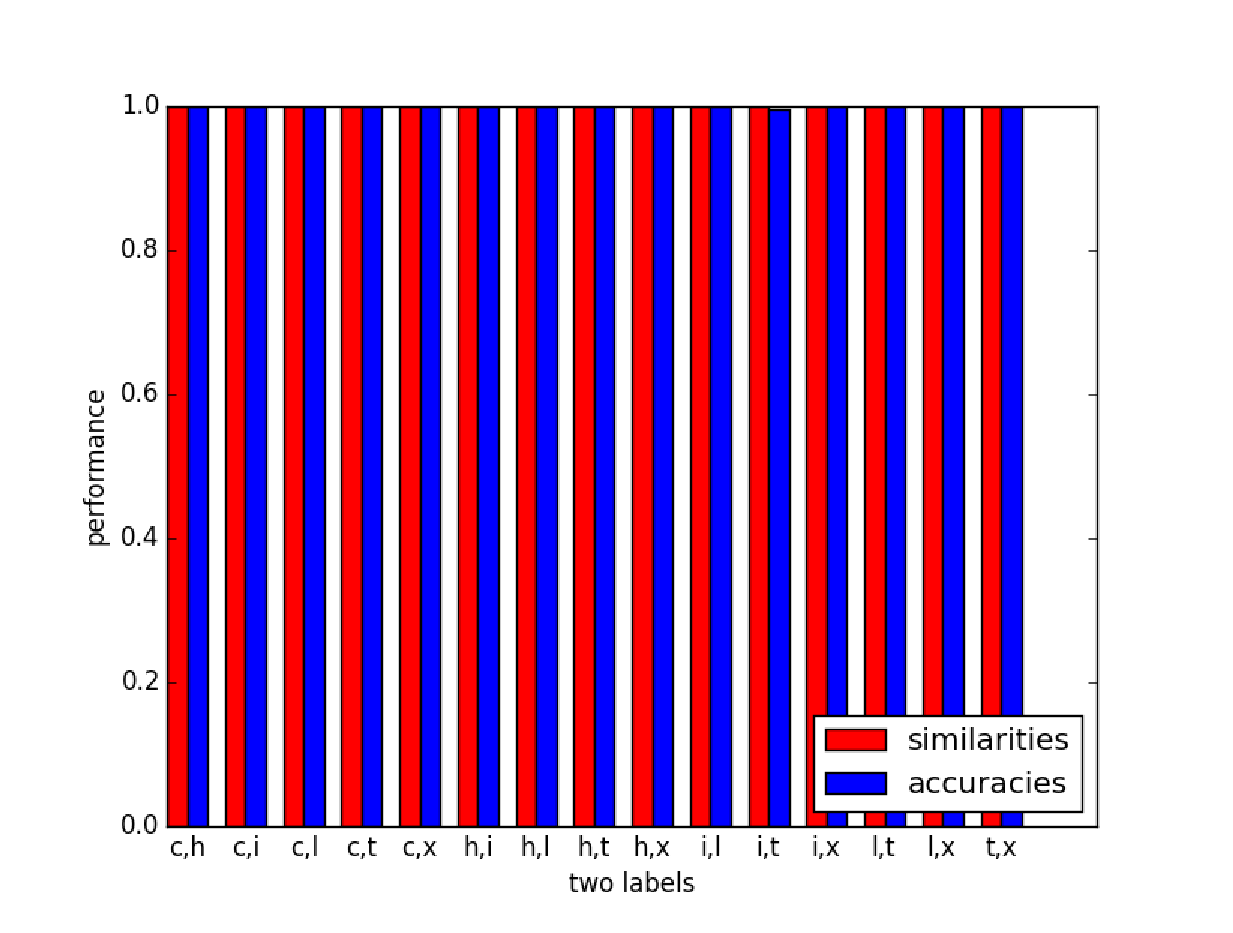
\includegraphics[width=\columnwidth]{figs/two_label_performance}
    \caption{2種類画像における識別性能}
    \label{fig:two-label-performance}
\end{figure}
%%% -------------------------------------------------


%%% -------------------------------------------------
\section{画像の種類数による想起性能変化}
画像の種類を2から6まで変化させ,想起性能の変化を調べた.
\ref{sec:two-label-performance}より,組み合わせによる性能の変動が小さいことから
アルファベット順に各種類数分を選択し性能変化を見ることとし,
性能テストの際に加えるノイズは5\%とした.

\figref{labels-performance}に示すように,画像の種類を増加させると概ね想起性能は下がるが,
図ではラベル数6の際に5と比べて性能値が上昇している.
このことから,画像の種類に対して想起性能は単調減少するわけではなく,
より多種の画像に対しても適応可能であると考えられる.
\begin{figure}[hbtp]
  \centering
    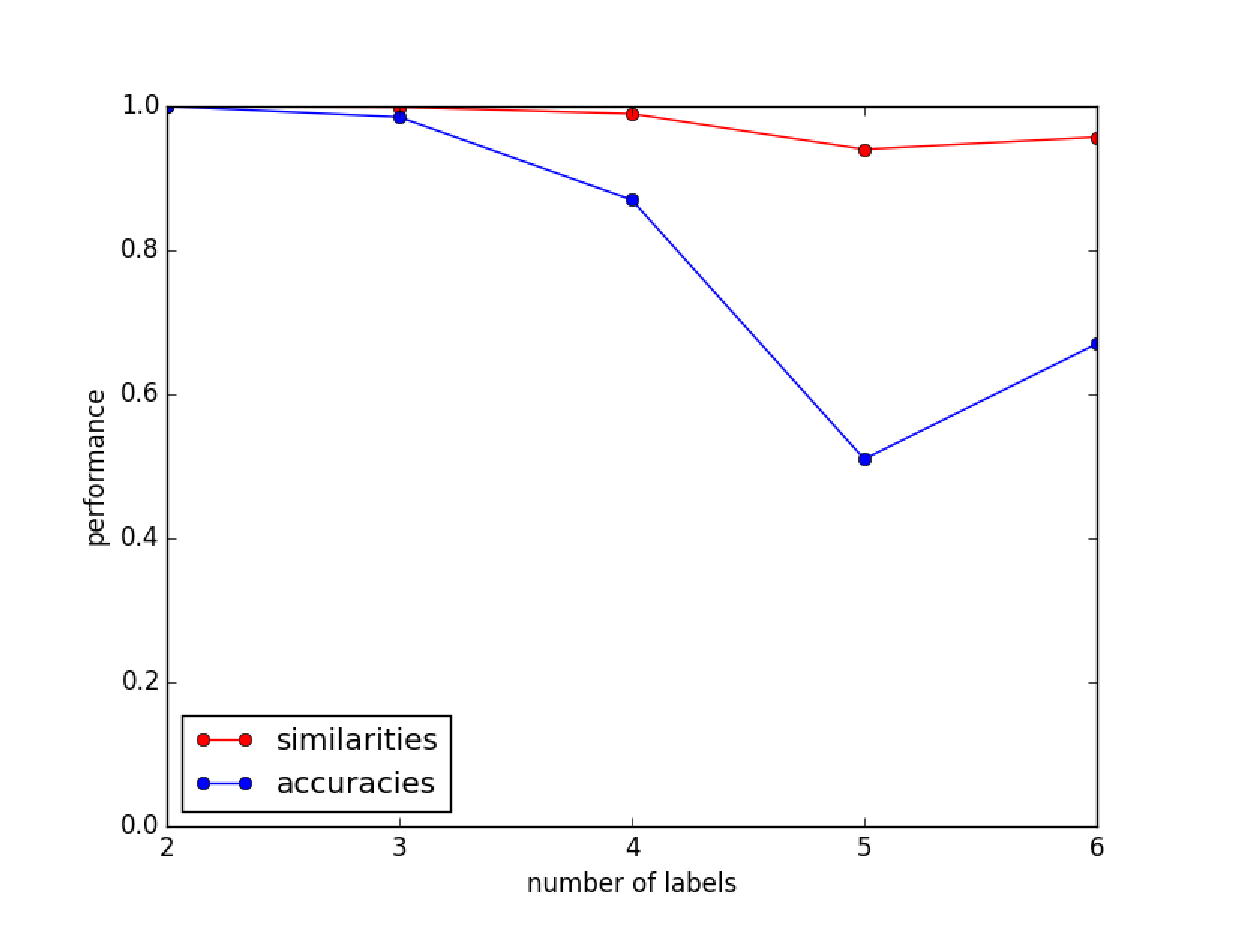
\includegraphics[width=\columnwidth]{figs/labels_performance}
    \caption{画像の種類数による想起性能変化}
    \label{fig:labels-performance}
\end{figure}
%%% -------------------------------------------------


%%% -------------------------------------------------
\section{入力画像のノイズ量による想起性能変化}
入力画像に加えるノイズ量を5から50\%まで変化させ,想起性能の変化を調べた.
画像の種類数は2, 4の場合とした.

結果は\figref{noise-performance}のようになり,
記憶させた画像種類数が2の場合には,入力画像に対するノイズは想起性能に大きな影響を与えることはなく,
50\%のノイズを加えた場合でもほぼ100\%の想起性能を持つ.

一方で画像種類数が4の場合には,ノイズの増加に従って想起性能は大きく減少した.
これは,\figref{noise-label4-wrong-sample}に示すように,
記憶画像の別の画像を想起してしまうことが起こりやすくなるからだと考えられる.

\begin{figure}[hbtp]
  \centering
    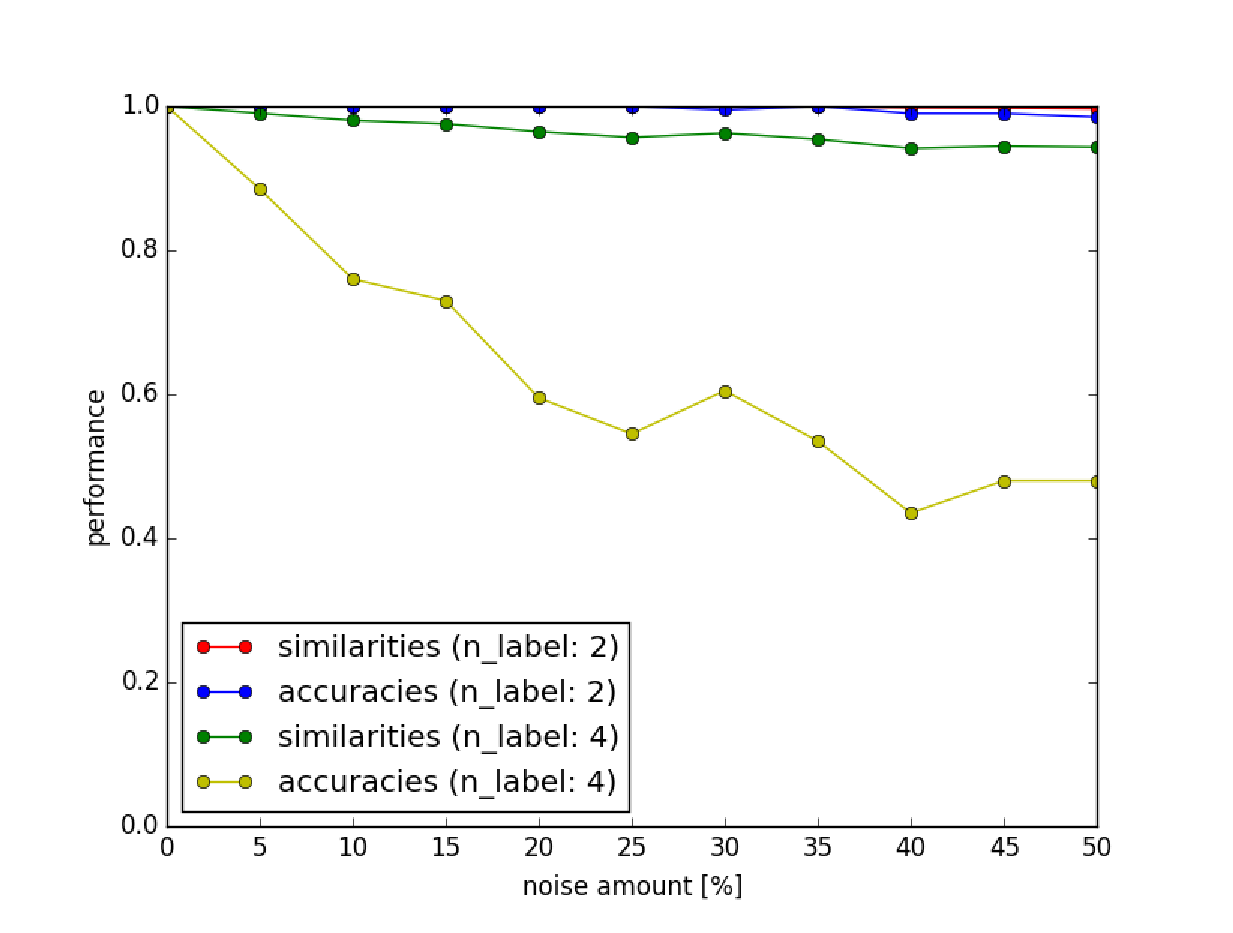
\includegraphics[width=\columnwidth]{figs/noise_performance}
    \caption{ノイズに対する想起性能変化}
    \label{fig:noise-performance}
\end{figure}

\begin{figure}[hbtp]
  \centering
    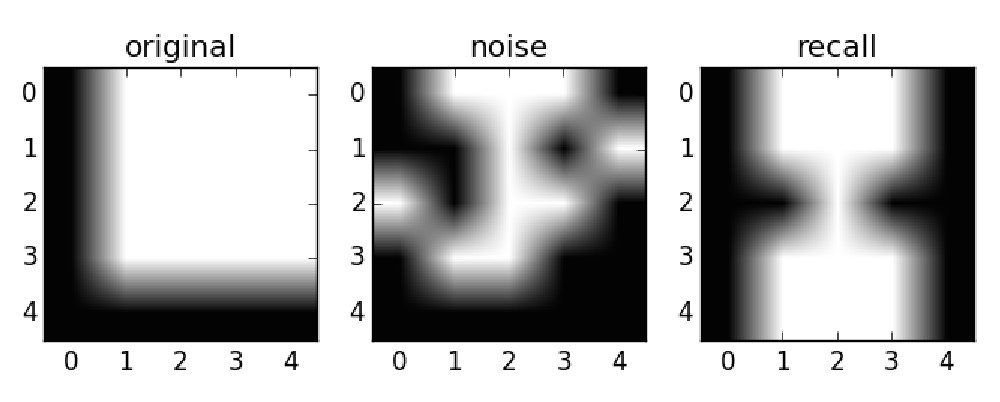
\includegraphics[width=\columnwidth]{figs/noise_label4_wrong_sample}
    \caption{画像種類数4でのノイズによる誤りの例}
    \label{fig:noise-label4-wrong-sample}
\end{figure}
%%% -------------------------------------------------


%%% Bibliography ------------------------------------
% \begin{thebibliography}{9}
%   \bibitem{bib1} Samuel R.Buss,"Introduction to Inverse Kinematics with Jacobian Transpose,Pseudoinverse and Damped Least Squares methods"
% \end{thebibliography}
%%% -------------------------------------------------


\end{document}
